% \iffalse meta-comment
% 
% Copyright (C) 2018 by M.J.W. Snippe
% -----------------------------------
% 
% This work may be distributed and/or modified under the
% conditions of the LaTeX Project Public License, either version 1.3
% of this license or (at your option) any later version.
% The latest version of this license is in
% 
%     http://www.latex-project.org/lppl.txt
% 
% and version 1.3 or later is part of all distributions of LaTeX
% version 2005/12/01 or later.
% 
% This work has the LPPL maintenance status `maintained'.
% 
% The Current Maintainer of this work is M.J.W. Snippe
% 
% This work consists of the files found at https://github.com/MaxSnippe/xbondgraphs.
% 
% \fi
% 
% \iffalse
%<package>\NeedsTeXFormat{LaTeX2e}[2018/04/01]
%<package>\ProvidesPackage{xbondgraphs}
%<package>    [2018/05/02 v0.0.1 Bond graph drawing using TikZ]
% 
%<*driver>
\documentclass{ltxdoc}
\usepackage{xbondgraphs}
\usepackage{xspace}
\usepackage{mathpazo}
\usepackage{pifont}
\usepackage{iconix}
\usepackage{booktabs}
\usepackage{tabu}
\usepackage{longtable}
\usepackage{footnote}
\usepackage{subcaption}
\usepackage{listings}
\usepackage[numbered]{hypdoc}
\usepackage[noabbrev]{cleveref}
\usepackage{lstautogobble}
% 
\pgfmathsetlengthmacro{\multibondwidth}{30mm}
\pgfmathsetlengthmacro{\singlebondwidth}{12.5mm}
\pgfmathsetmacro{\barbangle}{40}
%
\hyphenation{bond-graphs x-bond-graphs}
\newcommand\textvtt[1]{{\normalfont\fontfamily{cmvtt}\selectfont #1}}
%
\makesavenoteenv{table}
%
\lstset{
	autogobble,
	tabsize=4,
	breaklines=true,
	basicstyle=\ttfamily\small,
	language=[LaTeX]Tex,
}
%
\usetikzlibrary{positioning}
%
\newcommand{\Tikz}{Ti\textit{k}Z\xspace}
\newcommand{\pgf}{PGF\xspace}
\newcommand{\xbondgraphs}{\textsf{xbondgraphs}\xspace}
\newcommand{\bondgraphs}{\textsf{bondgraphs}\xspace}
\let\origLaTeX\LaTeX
\def\LaTeX{\origLaTeX\xspace}
\def\cmark{\ding{51}}
\def\xmark{\ding{55}}
%
\captionsetup{labelfont=bf,font=small,labelsep=endash}
\captionsetup[subfigure]{font=footnotesize}
%
\tikzset{
	> = stealth,
	arrow tip demonstration/.style={red,opacity=.75},
	arrow tip line style/.style={gray!40!black,line width = 0.5pt},
	annotation style/.style={line width = .4pt,gray,text=black,<->},
}
%
\EnableCrossrefs
\CodelineIndex
\RecordChanges
\begin{document}
	\DocInput{xbondgraphs.dtx}
\end{document}
%</driver>
% \fi
%
% \CheckSum{0}
%
% \CharacterTable
%  {Upper-case \A\B\C\D\E\F\G\H\I\J\K\L\M\N\O\P\Q\R\S\T\U\V\W\X\Y\Z
%   Lower-case \a\b\c\d\e\f\g\h\i\j\k\l\m\n\o\p\q\r\s\t\u\v\w\x\y\z
%   Digits \0\1\2\3\4\5\6\7\8\9
%   Exclamation \! Double quote \" Hash (number) \#
%   Dollar \$ Percent \% Ampersand \&
%   Acute accent \’ Left paren \( Right paren \)
%   Asterisk \* Plus \+ Comma \,
%   Minus \- Point \. Solidus \/
%   Colon \: Semicolon \; Less than \<
%   Equals \= Greater than \> Question mark \?
%   Commercial at \@ Left bracket \[ Backslash \\
%   Right bracket \] Circumflex \^ Underscore \_
%   Grave accent \‘ Left brace \{ Vertical bar \|
%   Right brace \} Tilde \~}
%
% \changes{v0.0.1}{2018/05/02}{Initial version}
%
% \GetFileInfo{xbondgraphs.sty}
%
% \DoNotIndex{\#,\$,\%,\&,\@,\\,\{,\},\^,\_,\~,\ }
% \DoNotIndex{\if,\else,\fi,\def,\ifcase,\or}
%
% \title{\xbondgraphs\thanks{This document corresponds to \xbondgraphs{}\space\fileversion, dated\space\filedate.} -- drawing bond graphs using \Tikz}
% \author{Marcus J.W. Snippe\thanks{E-mail: \href{mailto:m.j.w.snippe@saxion.nl}{m.j.w.snippe@saxion.nl}}}
%
% \maketitle
%
% \begin{abstract}
%	When using the \xbondgraphs-package, the user is able to draw visually pleasing bond graphs\footnote{\url{https://en.wikipedia.org/wiki/Bond_graph}}, while mostly maintaining the standard notation of \Tikz drawings. It defines two new \pgf arrows, an accompanying decoration to ensure the direction of the barb, as well as a \pgf shape for power (de-)mux elements. This package is based on the \bondgraphs package by G. Folkertsma\footnote{\url{https://ctan.org/pkg/bondgraphs}}, but does not (yet) cover all its functions. It \emph{might} result in more appealing bond graphs.
% \end{abstract}
% \tableofcontents
%\section{Introduction}
%	
%	\subsection{Motivation}
%		This package is a by-product of a project in which I was in need of a convenient way to draw bond graphs. At first, the \bondgraphs package was sufficient, but as the delivery date of the final report approached, I became less and less satisfied by the aesthetic end result of my bond graphs, especially when using multi-bonds. \Cref{fig:comparisonmultibonds} shows a simple comparison between the \bondgraphs- and the \xbondgraphs package.
%		
%		\begin{figure}[htbp]
	%			\centering
	%			\begin{subfigure}{.45\linewidth}
		%				\centering
		%				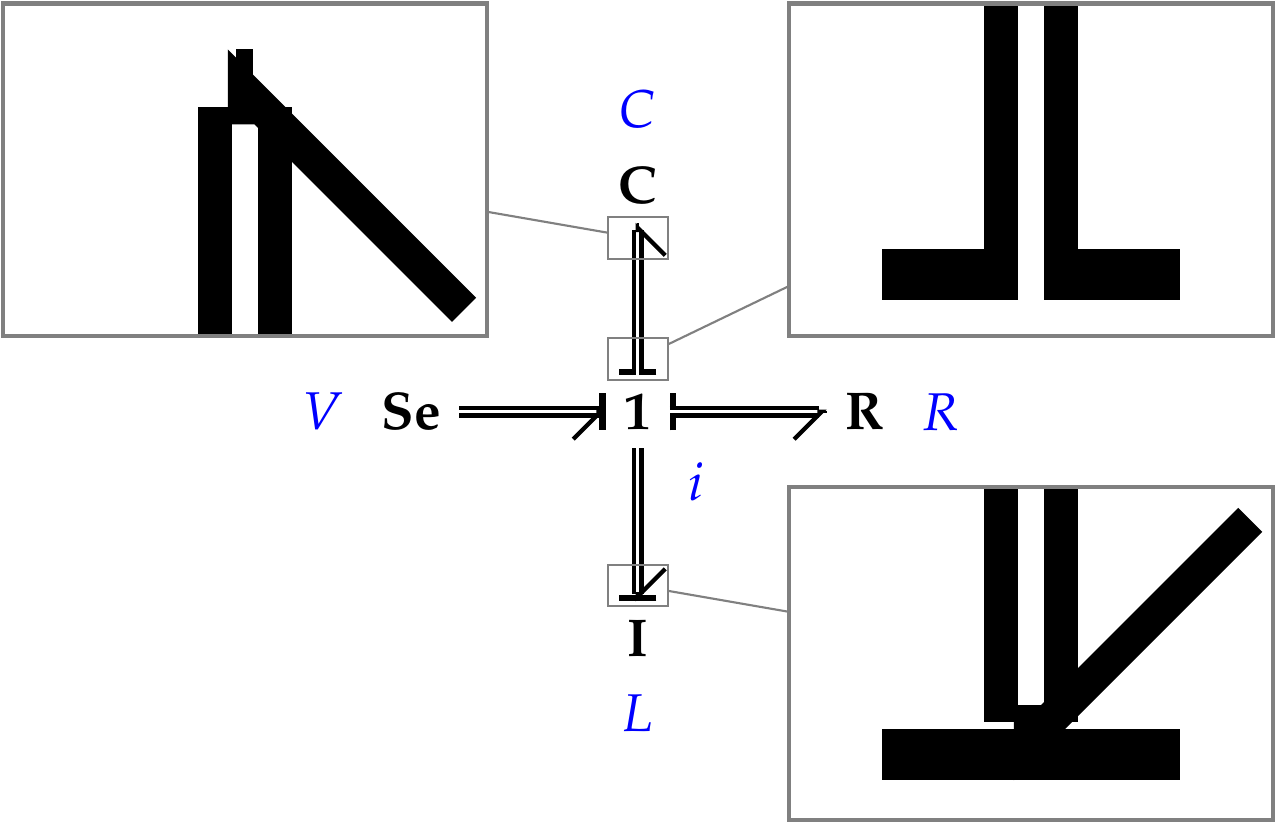
\includegraphics[scale=1.5]{src/bondgraphs_example.pdf}
		%				\caption{Using the \bondgraphs package}
		%				\label{fig:comparisonmultibonds-bondgraphs}
		%			\end{subfigure}
	%			\begin{subfigure}{.45\linewidth}
		%				\centering
		%				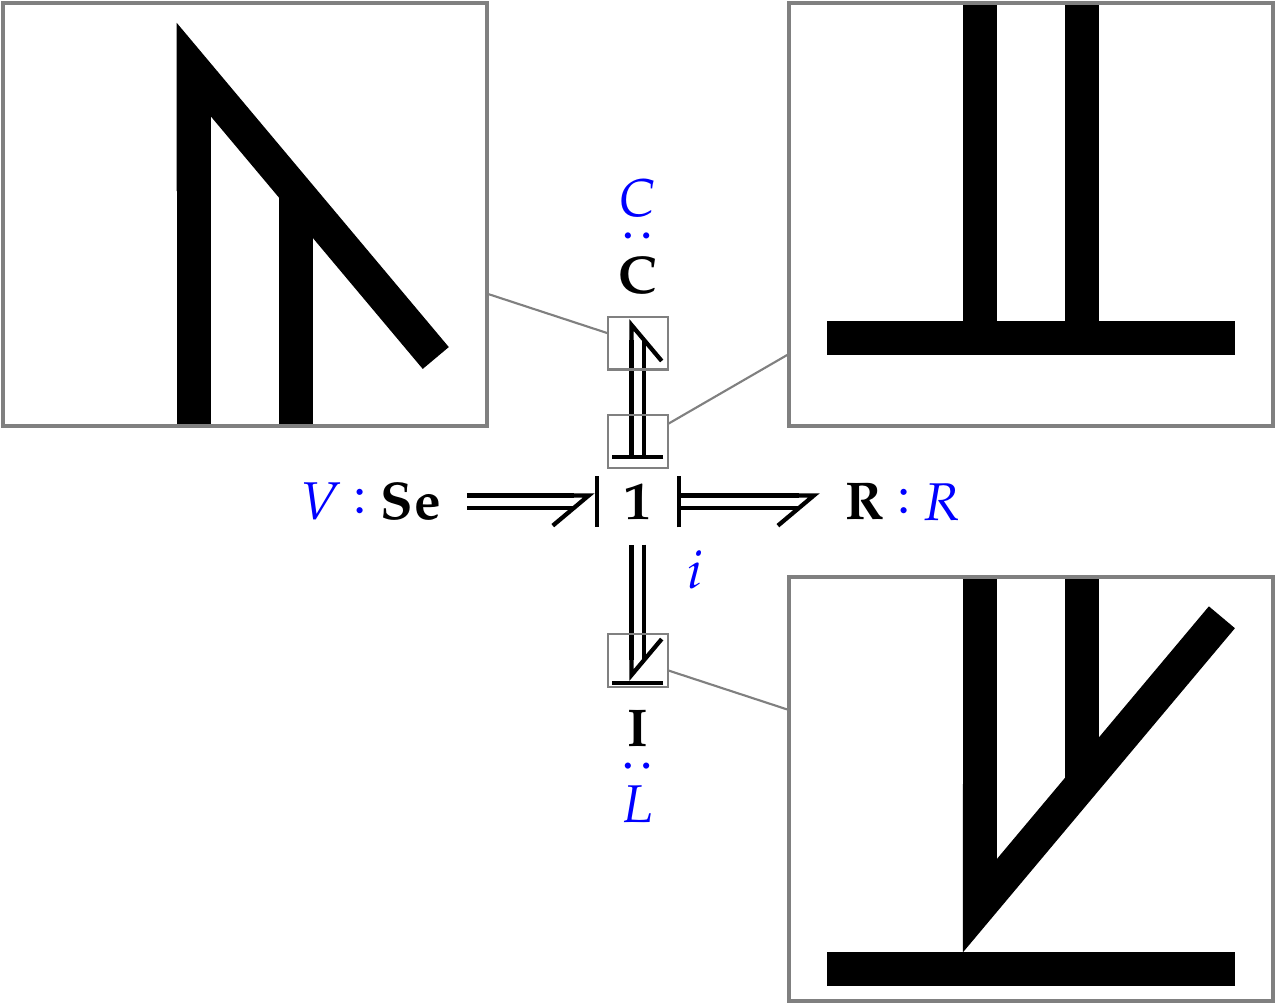
\includegraphics[scale=1.5]{src/xbondgraphs_example.pdf}
		%				\caption{Using the \xbondgraphs package}
		%				\label{fig:comparisonmultibonds-xbondgraphs}
		%			\end{subfigure}
	%			\caption{Comparison of multi bond graph drawing.}
	%			\label{fig:comparisonmultibonds}
	%		\end{figure}
%		
%		\Cref{fig:comparisonmultibonds} shows the main motivation for this package. Although of course subjective, most of the differences between the \bondgraphs- and the \xbondgraphs package can be argued to be improvements. The drawing in \cref{fig:comparisonmultibonds-xbondgraphs} is overall more consistent. %The causality stroke of \cref{fig:comparisonmultibonds-bondgraphs} with flow-out causality is overdrawn by the inner line of the multi bond. This is fixed in \cref{fig:comparisonmultibonds-xbondgraphs}.
%		Most flaws of the drawing in \cref{fig:comparisonmultibonds-bondgraphs} can be traced back to the decoration being a \texttt{postaction}. This however is needed to inherit other options from the \verb|\draw|-command, e.g. color.
%		
%		Due to these reasons, I wrote the \xbondgraphs package from scratch, re-using some parts but in a completely different setup.
%		
%	\subsection{Alternatives}
%	
%		As already mentioned, this package is based on the \bondgraphs package, but does not (yet) cover all its functions. A comparison of main package functions is shown in \cref{tab:functioncomparison}.
%		
%		\begin{table}[h]
%			\centering
%			\caption{Function comparison between \bondgraphs and \xbondgraphs.}
%			\label{tab:functioncomparison}
%			\begin{tabular}{lcc}
%				\toprule
%				                                                                   &        \bondgraphs         &       \xbondgraphs        \\ \midrule
%				Automatic arrow barb direction                                     & \textcolor{green}{\cmark}  & \textcolor{green}{\cmark} \\
%				Single bond drawings                                               & \textcolor{green}{\cmark}  & \textcolor{green}{\cmark} \\
%				Multi bond drawings\footnote{See \cref{fig:comparisonmultibonds}.} & \textcolor{orange}{\cmark} & \textcolor{green}{\cmark} \\
%				Power (de-)mux element                                             &  \textcolor{red}{\xmark}   & \textcolor{green}{\cmark} \\
%				Multi-segment bonds                                                &  \textcolor{red}{\xmark}   & \textcolor{green}{\cmark} \\
%				Curly bond barb                                                    & \textcolor{green}{\cmark}  &  \textcolor{red}{\xmark}  \\
%				Colon between element and variable\footnote{This is optional.}     &  \textcolor{red}{\xmark}   & \textcolor{green}{\cmark} \\ \bottomrule
%			\end{tabular}
%		\end{table}
%		
%		A second alternative is the \textvtt{bondgraph}\footnote{\url{https://ctan.org/pkg/bondgraph}} package, but because it has nearly no documentation and an incomprehensible example file, I have never tried it personally.
%		
%	\subsection{Known issues}
%		
%		\begin{itemize}
%			\item None yet, but please submit issues to \url{https://github.com/MaxSnippe/xbondgraphs/issues}.
%		\end{itemize}
%\section{Basic usage}
%	
%	\subsection{Installation}
%		This package has not yet been included in popular \LaTeX distributions, and therefore can be installed only by downloading the source (\texttt{xbondgraphs.sty}) from \href{https://github.com/MaxSnippe/xbondgraphs}{the GitHub repository}\footnote{\url{https://github.com/MaxSnippe/xbondgraphs}} to your local TEXMF tree. It should be placed under \textvtt{\$TEXMF\$/tex/latex/local}.
%	
%	\subsection{Including the package}
%	\DescribeMacro{\usepackage\oarg{options}\marg{xbondgraphs}}
%		The package can be included with the well-known \lstinline|\usepackage[<options>]{xbondgraphs}|, where \meta{options} can be any of the options mentioned in \cref{sec:globaloptions}. Options that set the same keys to different values are treated in the order in which they are provided. The package works fine straight-out-of-the-box without setting any options.
%		
%	\subsection{Simple example}
%		A simple example of an electric domain dynamic model shown as an iconic diagram, and its domain independent equal model shown as a bond graph.
%		\begin{figure}[h]
%			\centering
%			\begin{subfigure}[t]{.48\linewidth}
%				\centering
%				\begin{tikzpicture}
%				\draw[line width=1pt] (-1,-1) 
%					-- ++(0,0.5)
%					-- node[voltage source,label={above:$ u $}]{} ++(0,1)
%					-- node[current,label={above:$ i $}]{} ++(0,0.5)
%					-- node[inductor,label={above:$ L $}]{} ++(2,0) 
%					-- node[resistor2,label={above:$ R $}]{} ++(0,-2) 
%					-- node[capacitor,label={above:$ C $}]{} cycle;
%				\path (-2.5,-2.25) rectangle (2.5,2.25);
%				\end{tikzpicture}
%				\caption{}
%			\end{subfigure}
%			\begin{subfigure}[t]{.48\linewidth}
%				\centering
%				\begin{tikzpicture}
%					\node (u) at (-1.5, 0.0) [bond graph element={Se}{},pin={left:$ u $}];
%					\node (i) at ( 0.0, 0.0) [bond graph element={1}{},label={300:$ i $}];
%					\node (c) at ( 0.0, 1.5) [bond graph element={C}{},pin={above:$ C $}];
%					\node (r) at ( 1.5, 0.0) [bond graph element={R}{},pin={right:$ R $}];
%					\node (l) at ( 0.0,-1.5) [bond graph element={L}{},pin={below:$ L $}];
%					\draw[bond={effort out}] (u) -- (i);
%					\draw[bond={effort in}] (i) -- (c);
%					\draw[bond={effort in}] (i) -- (r);
%					\draw[bond={effort out}] (i) -- (l);
%					\path (-2.5,-2.25) rectangle (2.5,2.25);
%				\end{tikzpicture}
%				\caption{}
%			\end{subfigure}
%%			\begin{subfigure}{.31\linewidth}
%%				\begin{tikzpicture}[line width=1pt]
%%					\node[mechanical earth,minimum height = 3cm] at (0,-1){};
%%					\draw (0,0) -- ++(1.5,0) node[spring,label={above:$ \frac{1}{C} $}]{};
%%					\draw (0,-1) -- ++(1.5,0) node[damper,label={above:$ R $}]{};
%%					\draw (0,-2) -- ++(1.5,0) node[forcesource2,label={above:$ u $}]{};
%%					\node[mass2,minimum height = 3cm, minimum width = 2cm,label={south:$ L $}](m) at (2.5,-1){};
%%					\draw[->>,>=stealth] (m.north) -- ++(0,.5) -- ++(.5,0) node[component,label={east:$ i $}]{};
%%				\end{tikzpicture}
%%			\end{subfigure}
%			\caption{Electric domain dynamic model and its bond graph representation.}
%		\end{figure}
%\section{Options}
%	
%	\subsection{Global (package) options}
%		\label{sec:globaloptions}
%		
%		\DescribeMacro{barbdirection}
%		
%		\begin{tikzpicture}
%			\foreach \angle in {0,30,...,359}{
%				\draw[bond,/XBG/barbdirection=leftbelow] (0,0) -- ++(\angle:1.25);
%				\draw[bond,/XBG/barbdirection=alwaysbelow] (2.5,0) -- ++(\angle:1.25);
%				\draw[bond={multi},/XBG/barbdirection=leftbelow] (5,0) -- ++(\angle:1.25);
%				\draw[bond={multi},/XBG/barbdirection=alwaysbelow] (7.5,0) -- ++(\angle:1.25);
%			}
%		\end{tikzpicture}
%		
%	\subsection{Local (\Tikz) options}
%		\label{sec:localoptions}
%\section{Arrow tips}
%	
%	\subsection{Single bond arrow tip}
%		
%		\begin{tikzpicture}
%			
%			% Calculate actual path points
%				\pgfmathsetlengthmacro{\tipx}{\singlebondwidth}
%				\pgfmathsetlengthmacro{\tipy}{0pt}
%				\pgfmathsetlengthmacro{\backx}{-1/tan(\barbangle)*(\multibondwidth-0.5*cos(\barbangle)*\singlebondwidth) + \singlebondwidth}
%				\pgfmathsetlengthmacro{\backy}{\multibondwidth - 0.5*cos(\barbangle)*\singlebondwidth}
%			% Calculate points of outer dimensions as needed by pgf
%				\pgfmathsetlengthmacro{\hullpointx}{\backx + 0.5*\singlebondwidth*sin(\barbangle)}
%				\pgfmathsetlengthmacro{\hullpointy}{\multibondwidth}
%				\pgfmathsetlengthmacro{\tipendx}{0.5*\singlebondwidth/tan(\barbangle/2) + \tipx}
%				\pgfmathsetlengthmacro{\tipendy}{-0.5*\singlebondwidth}
%			
%			\begin{scope}[line width = \singlebondwidth,/XBG/multibondwidth=\multibondwidth]
%			% Existing line
%			\draw (0,0) -- (-5,0);
%			
%			% Arrow tip
%			\draw[arrow tip demonstration,-{Single Bond Barb[left].|[width=2*\multibondwidth]}] (0,0) -- (\tipendx+\singlebondwidth,\tipy);
%	%					\draw[arrow tip demonstration] (0,0) -- (\tipx,\tipy) -- (\backx,\backy);
%	%					\draw[arrow tip demonstration] (\tipendx+0.5*\singlebondwidth,-\multibondwidth) -- (\tipendx+0.5*\singlebondwidth,\multibondwidth);
%			\draw[arrow tip line style] (0,0) -- (\tipx,\tipy) -- (\backx,\backy);
%			\end{scope}
%			
%			\begin{scope}[annotation style]
%				\begin{scope}[xshift=\tipendx+2.5mm]
%					\draw (0,\tipendy) -- node[right]{$ y_a $} (0,\tipy);
%					\draw (0,\tipy) -- node[right]{$ y_b $} (0,\backy);
%					\draw (0,\backy) -- node[right]{$ y_c $} (0,\hullpointy);
%				\end{scope}
%				\begin{scope}[yshift=\hullpointy+2.5mm]
%					\draw (\backx,0) -- node[above]{$ x_a $} (\hullpointx,0);
%					\draw (\hullpointx,0) -- node[above]{$ x_b $} (0,0);
%					\draw (0,0) -- node[above]{$ x_c $} (\tipx,0);
%					\draw (\tipx,0) -- node[above]{$ x_d $} (\tipendx,0);
%				\end{scope}
%			\end{scope}
%			
%			\begin{scope}[help lines]
%			\draw (\backx,\hullpointy) -- (\hullpointx,\hullpointy-|\tipendx+3mm,0);
%			\draw (\tipx,\tipy) -- (\tipx,\tipy-|\tipendx+3mm,0);
%			\end{scope}
%			
%		\end{tikzpicture}
%		
%	\subsection{Multi bond arrow tip}
%		
%		\begin{tikzpicture}
%			
%			% Calculate actual path points
%				\pgfmathsetlengthmacro{\startx}{0pt}
%				\pgfmathsetlengthmacro{\starty}{-0.5*\multibondwidth+0.5*\singlebondwidth}
%				\pgfmathsetlengthmacro{\tipx}{(\multibondwidth-\singlebondwidth)/tan(\barbangle)}
%				\pgfmathsetlengthmacro{\tipy}{-0.5*\multibondwidth + 0.5*\singlebondwidth}
%				\pgfmathsetlengthmacro{\backy}{1.5*\multibondwidth - 0.5*\singlebondwidth*cos(\barbangle)}
%				\pgfmathsetlengthmacro{\backx}{-(\backy+\tipy)/tan(\barbangle)}
%			% Calculate points of outer dimensions as needed by pgf
%				\pgfmathsetlengthmacro{\hullpointx}{\backx + 0.5*\singlebondwidth*sin(\barbangle)}
%				\pgfmathsetlengthmacro{\hullpointy}{1.5*\multibondwidth}
%				\pgfmathsetlengthmacro{\tipendx}{0.5*\singlebondwidth/tan(\barbangle/2) + \tipx}
%				\pgfmathsetlengthmacro{\tipendy}{-0.5*\multibondwidth}
%			
%			\begin{scope}[line width = \singlebondwidth]
%				% Existing line
%				\draw (0,\starty) -- (-5,\starty); 
%				\draw (0,-\starty) -- (-5,-\starty); 
%				
%				% Arrow tip
%				%					\draw[double,double distance={\multibondwidth-2*\singlebondwidth},arrow tip demonstration,-{Multi Bond Barb[left].|[width=3*\multibondwidth]}] (0,0) -- (\tipendx+\singlebondwidth,0);
%				\draw[arrow tip demonstration] (\startx,\starty) -- (\tipx,\tipy) -- (\backx,\backy);
%				\draw[arrow tip line style] (\startx,\starty) -- (\tipx,\tipy) -- (\backx,\backy);
%				\draw[arrow tip line style,green] (\tipx,\tipy) -- ++ (180-\barbangle:10cm);
%			\end{scope}
%			
%			\node[draw,cross out] at (\hullpointx,\hullpointy){};
%			
%			\begin{scope}[annotation style]
%				\draw[<->] (\tipx+5mm,\tipy) -- node[right]{$ 2a $} ++ (0,2*\multibondwidth);
%				\draw[<->] (\startx,\starty-5mm) -- node[below]{} (\tipx,\tipy-5mm);
%			\end{scope}
%			
%		\end{tikzpicture}
%\section{Examples}
%	
%	\begin{tikzpicture}
%		\node (Vabc) at (0,0) [bond graph element={MSe}{},label={west:$ V_{abc} $}];
%		\node (iabc) [right=of Vabc,bond graph element={1}{},label={300:$ i_{abc} $}];
%		\node (Rs) [above=of iabc,bond graph element={R}{},pin={north:$ R_s $}];
%		\node (Ls) [below=of iabc,bond graph element={L}{},pin={south:$ L_s $}];
%		\node (Klambda) [right=of iabc,bond graph element={MGY}{},pin={south:$ K\Lambda(\theta_e) $}];
%		\node (mux1) [right=of Klambda,mux={outputs=3}];
%		\node (omegae) [right=of mux1,bond graph element={1}{},label={300:$ \omega_e $}];
%		\node (1overp) [right=of omegae,bond graph element={TF}{},pin={south:$ \frac{1}{p} $}];
%		\node (omegam) [right=of 1overp,bond graph element={1}{},label={300:$ \omega_m $}];
%		\node (Dr) [above=of omegam,bond graph element={R}{},pin={north:$ D_r $}];
%		\node (Jr) [below=of omegam,bond graph element={I}{},pin={south:$ J_r $}];
%	%			\node (taum) [right=of omegam,bond graph element={p}{},label={east:$ \tau_m $}];
%		
%		\begin{scope}[bond={multi}]
%			\draw[bond={effort out}] (Vabc) -- (iabc);
%			\draw[bond={effort in}] (iabc) -- (Rs);
%			\draw[bond={effort out}] (iabc) -- (Ls);
%			\draw[bond={effort in}] (iabc) -- (Klambda);
%			\draw[bond={effort out}] (Klambda) -- (mux1);
%		\end{scope}
%		
%		\foreach \i in {1,2,3}{
%			\draw[bond={effort out}] (mux1.output\i) -- ++ (0.8,0) -- (omegae);
%		}
%		\draw[bond={effort out}] (omegae) -- (1overp);
%		\draw[bond={effort out}] (1overp) -- (omegam);
%		\draw[bond={effort out}] (omegam) -- (Jr);
%		\draw[bond={effort in}] (omegam) -- (Dr);
%	%			\draw[bond={effort in}] (omegam) -- (taum);
%	\end{tikzpicture}